\chapter{Project overview}
\section*{Introduction}
The approach to our work on this project is detailed in this report, which is structured around six chapters.\\

The first chapter introduces the general context of the project, we will start with the presentation of the organization that welcomed us for our internship, then we will continue with a study of the existing situation and its critique. Then we will go on to the presentation of our project and we will end by the choice of the work methodology we will adopt.  \\

The second chapter entitled "Requirements analysis" will represent the preliminary phase, which revolves around the analysis and specification of needs in order to formalize the functionalities of our future system and the various constraints to be respected during its implementation. 

The third chapter  will be dedicated to clarify the basic notions on which our project is based, namely the presentation of the integrated management software packages.\\

The fourth, fifth and sixth chapters will be dedicated to the realization of the different modules of our project. They will include the detailed design as well as the interfaces of our final increment explained by the process of their realization. 

% Une section

% Exemple d'une section qui porte une référence à une bibliographie
% NB: il faut bien suivre le syntaxe pour ne pas tomber dans le cas où il y a une référence dans la table des matières.
\section{Presentation of the host company}
VatoSmart is an engineering and consulting start-up, specialized in research and development of IT solutions, operating in various fields of information technology and located in the Technology Pole el Ghazela since 2018.\\
Wishing to offer a better service to its customers, VatoSmart adopts a strategic approach reflecting the spirit of commitment and determination in order to develop a relationship of trust and partnership with its customers and to be well positioned in a market in perpetual movement.   \\
The team is strongly involved in the life of the company, and endowed with a sense of innovation and know-how, which guarantees the quality of the deliverable and the satisfaction of its customers. \\
Since its creation, the VatoSmart team has been dedicated to supporting its clients in the implementation of information systems that are perfectly adapted to their needs, as well as consulting in both telecommunication and marketing.
\begin{itemize}
\item Information systems: the start-up has chosen Odoo open-source ERP for the design of optimal and efficient information systems to centralize the management of the client's different functional processes such as the administration of the organization, human resources management, invoicing, stock management and so on. 


\item Marketing: VatoSmart accompanies its clients from the study to the implementation of digital marketing campaigns.
\end{itemize}

\section{Presentation of the project}


\subsection{Project description}
Our solution allows you to independently and efficiently manage business travel within your company. It is a Travel Order Engine allowing you to book, manage your invoices and payments, define your travel policies and rules for your employees, all in one place. With real-time reporting and tracking, you will keep control of your expenses.
\subsection{Problematic}
Currently, our client relies on paper files and excel sheets to coordinate and process all of their business travels.\\
And that raises some problems from which are :
\begin{itemize}
\item The agents lose an insatiable amount of time just by having to go through all physical documents looking for files
\item Calculating Per diem and other policies is done by hand and requires double-checking.
\item Documents that are related to employees are valuable and contain personal information. These data are unfortunately scattered in archive boxes, which increases the risk of their loss and breaks the principle of securing the employee's information.
\end{itemize}
\subsection{Provided Solution}
In this project we propose to develop and implement three modules:
\begin{itemize}
\item Configuration module: this is a parameterization module dedicated to the administrators which allows parameterizing the activity of the platform.  
\item Employee management module: dedicated to the management of the company's departments and the employee's information as well as the hierarchy.
\item travel order management module: this is a module that manages the travel orders' workflow.
\end{itemize}





\section{Methodological choice}
In this section, we discuss the modeling language for the design of the
project and the methodology for its realization.
\subsection{Methodology}
Methodology is the systematic, theoretical analysis of the methods applied to a field of study.\cite{Methodology}\\
We opted for the Agile SCRUM methodology to manage our project as efficiently as possible\\
SCRUM is based on the principles of transparency to all stakeholders along with continuous inspection and adaptation to changing conditions. These result in a methodology embracing change and promoting an environment where all members of the project team share an equal voice regarding how the application will deliver value to its users.\\
Scrum has several advantages:\\
- The team gets a clear visibility of the project's progress.\\
- Requirements are prioritized according to the needs.\\
- Large projects are divided into easily manageable sprints.\\
    \begin{figure}[htpb]
    \centering
    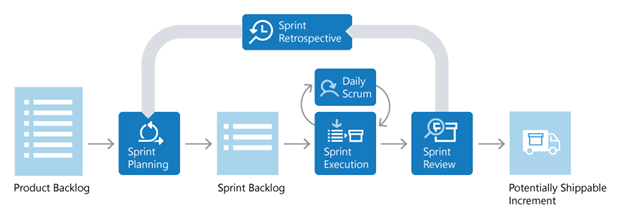
\includegraphics[scale=0.65]{img/scrumLifeCycle.png}
    \caption{The Scrum Life Cycle}
\end{figure}
\subsection{Modelization}
we have opted for the UML modeling language that
allows the description and visualization of needs, as well as the definition of the software architecture.\\
We present the diagrams useful for the design of the project :\\
- Class diagram to define the structure of the application.\\
- Use case diagram to visualize thebehavior of the application.\\
- Sequence diagram to describe the different interactions between actors and various system components.\\


\section*{Conclusion}
    This chapter provided an overview of the general context of our end-of-study project. First of all we presented the agency "VatoSmart" which is the host organization of our internship. Then we presented the problem we propose to solve. We continued with a study of the existing situation and its criticism which allowed us to identify the objective of our project and our motivation and we finally chose a working methodology.
In what follows we will begin a study of requirements that will allow us to clarify some important notions.   